% Asset ID: AS1AlgebraicExpressionsTIKZ-001
% Source: Dr Frost Algebraic Expressions index notation slide and transcript
% Related lesson section: Key Definitions and Notation
% Purpose: Label base, exponent/index and power notation for 3^5.

\documentclass[tikz,border=8pt]{standalone}
\usetikzlibrary{arrows.meta,positioning,calc}

\begin{document}
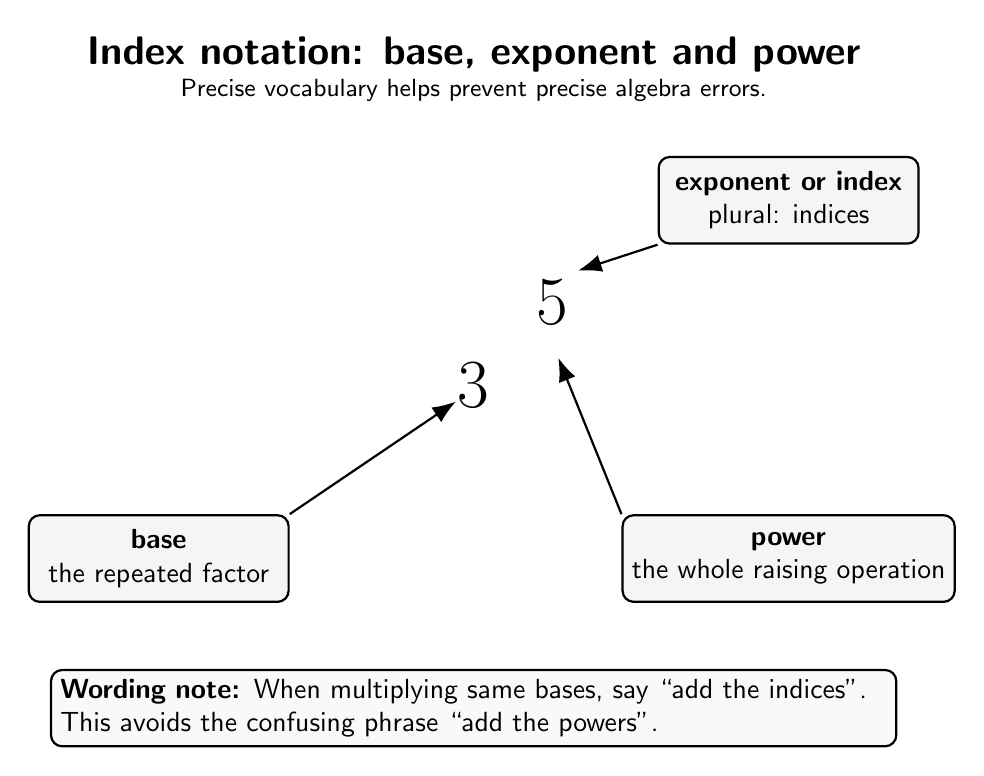
\begin{tikzpicture}[
    font=\sffamily,
    arrow/.style={-{Latex[length=3mm]}, thick},
    labelbox/.style={draw, rounded corners=4pt, thick, fill=gray!8, align=center, minimum width=3.3cm, minimum height=1.1cm}
]

\node[align=left, font=\sffamily\bfseries\Large] at (0,4.2)
{Index notation: base, exponent and power};
\node[align=left, font=\sffamily\small] at (0,3.75)
{Precise vocabulary helps prevent precise algebra errors.};

\node[font=\fontsize{64}{70}\selectfont] (base) at (0,0) {$3$};
\node[font=\fontsize{36}{40}\selectfont] (index) at (1.0,1.05) {$5$};

\node[labelbox] (baseLabel) at (-4,-2.2) {\textbf{base}\\the repeated factor};
\node[labelbox] (indexLabel) at (4,2.35) {\textbf{exponent or index}\\plural: indices};
\node[labelbox] (powerLabel) at (4,-2.2) {\textbf{power}\\the whole raising operation};

\draw[arrow] (baseLabel.north east) -- ($(base.south west)+(0.1,0.2)$);
\draw[arrow] (indexLabel.south west) -- (index.north east);
\draw[arrow] (powerLabel.north west) -- ($(base.east)+(0.75,0.35)$);

\node[draw, rounded corners=4pt, thick, fill=gray!5, align=left, text width=10.5cm] at (0,-4.1)
{\textbf{Wording note:} When multiplying same bases, say ``add the indices''. This avoids the confusing phrase ``add the powers''.};

\end{tikzpicture}
\end{document}
